\section{Specific Requirement}

\subsection{External Interface Requirements}
\textit{SafeStreets} is a mobile based application, the following section will give a more detailed description, in terms of hardware, software and communication interfaces.
\subsubsection{User Interfaces}
    \textbf{Login} \newline When a Guest downloads SafeStreets for the first time, the first interface will be the login one. In \textit{Figure 4} it is also shown that if the Guest doesn't have an account it is possible to proceed by registering and creating a new account.\vspace{1cm}
    \begin{figure}[h]
        \centering
        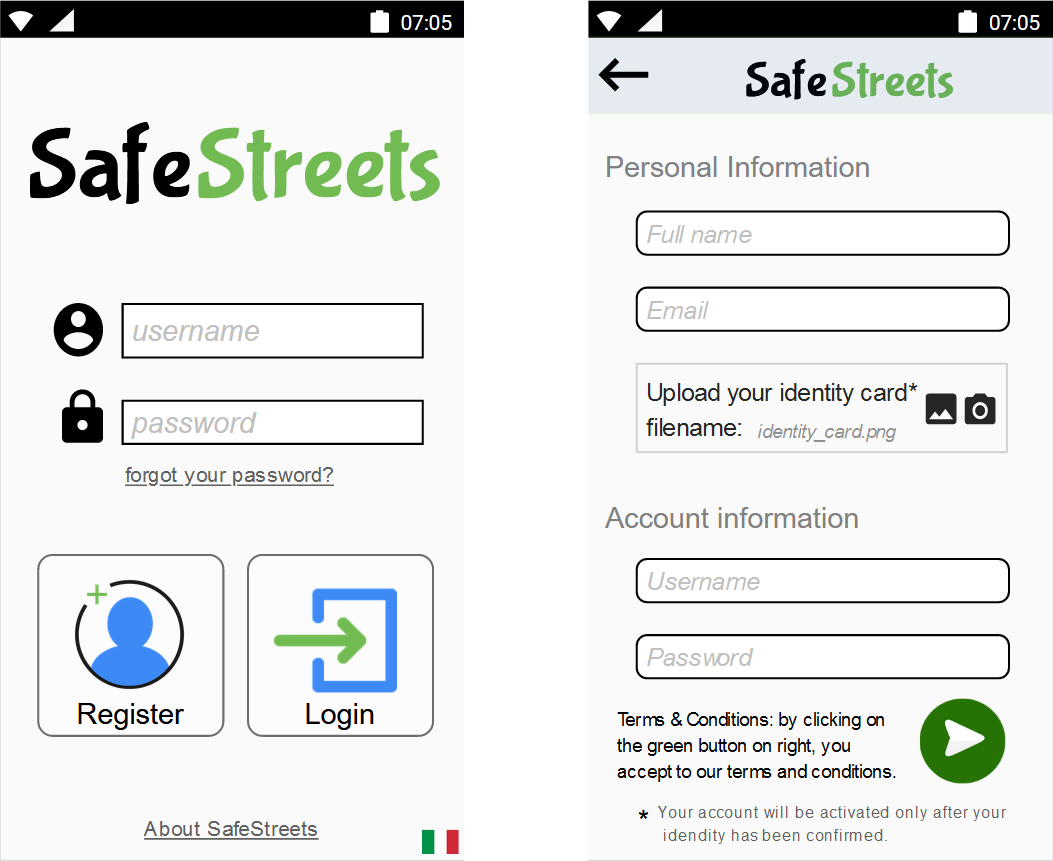
\includegraphics[scale=0.56]{Images/login_register.png}
        \caption{Login and Register interface}
    \end{figure}\newpage
    \noindent\textbf{Register}\newline
    In the register interface \textit{Figure 5}. It will be asked to the Guest to insert his/her personal information, to upload an Identification card (since it is required that all accounts must be authenticated) and to choose an \textit{Username} and a \textit{Password}.
    \\\\
        \begin{figure}[h]
    \centering
    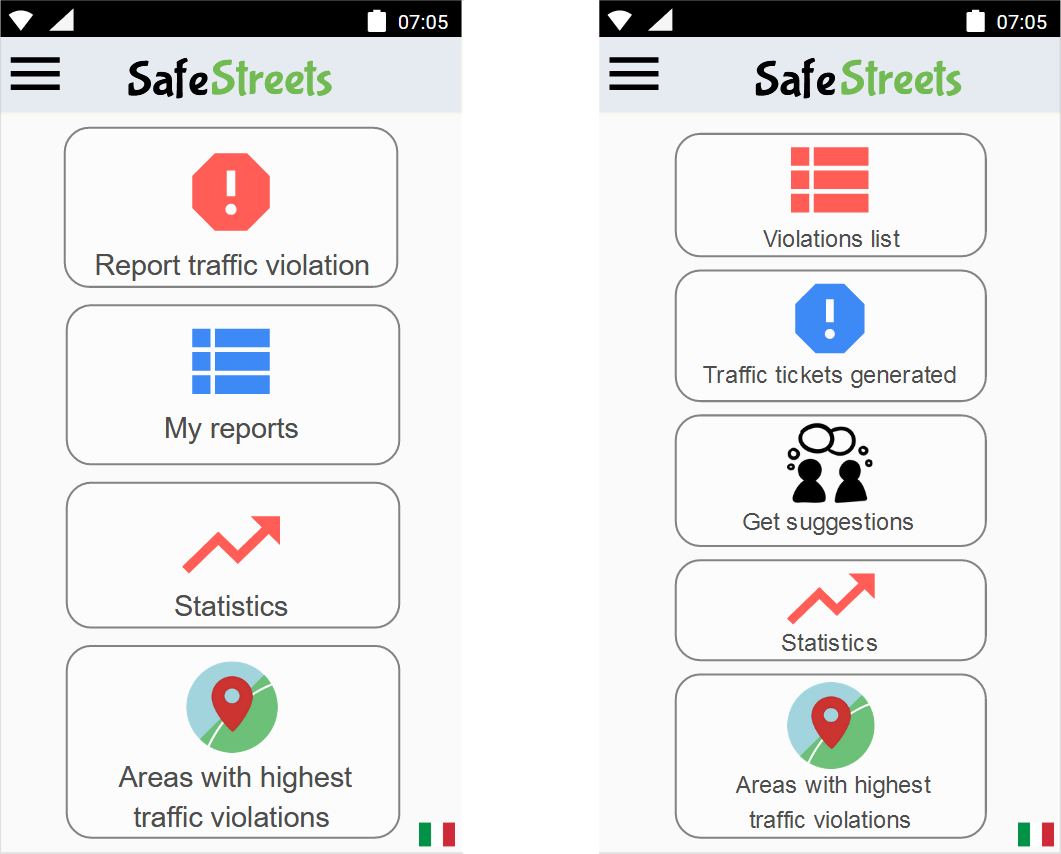
\includegraphics[scale=0.56]{Images/user_authority_menu.png}
    \caption{User and Authority Home Page interface}
    \end{figure}
    \newline
    \textbf{User Home Page}\newline
    This activity contains all the possible functionalities that a simple User can use. Thus, a User can:
    \begin{itemize}
        \item Report a Traffic Violation.
        \item View his/her own notifications sent to Authorities and their status.
        \item View statistics like the effectiveness of the application, the most egregious offenders, etc.
        \item Open a Map that shows safe and unsafe areas (with the option to use also the data from municipality).
    \end{itemize}
    \textbf{Authority Home Page}\newline
    For Authorities the functions available are a bit different, an authority can:
    \begin{itemize}
        \item Access to the notifications sent by users.
        \item View the traffic tickets generated.
        \item Get the suggestions elaborated by the application.
        \item View statistics like the effectiveness of the application, the most egregious offenders, etc.
        \item Open a Map that shows safe and unsafe areas (with the option to use also the data from municipality).
    \end{itemize}
    \vspace{5mm}
    \begin{figure}[h]
        \centering
        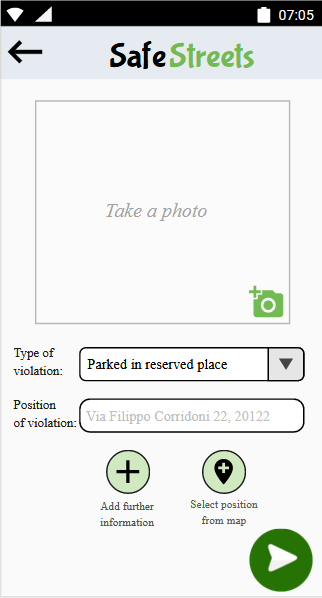
\includegraphics[scale=0.8]{Images/report_violation.png}
        \caption{Report traffic violation interface}
    \end{figure}
    \vspace{5mm}
    \textbf{Report a traffic violation}\newline
    This form allows users to notify authorities when traffic violations occur, an user takes a photo of the violation, selects the type of the violation and inserts the location where it occurred. Moreover, the User can also include further information about the vehicle like the license plate, the model, etc.
    \newpage
    \begin{figure}[h]
        \centering
        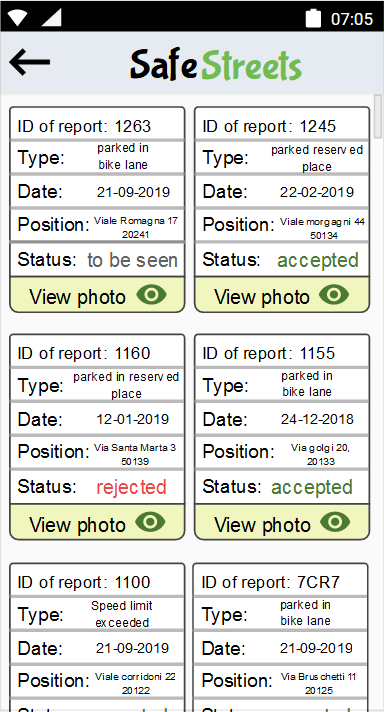
\includegraphics[scale=0.8]{Images/my_reports.png}
        \caption{My reports interface}
    \end{figure}
    \vspace{4mm}
    \noindent\textbf{My Reports}\newline
    Once a User sent a notification it is possible to see all the notifications sent to authorities, \textit{Figure 7}. In this activity it is also possible to search them by their ID and see their status. There are three possible status: to be seen, accepted, rejected.
        \newline\\
    \noindent\textbf{Violations list}\newline
    An Authority is able to see all the violations sent by users, the list shows the most important information to know if an Authority is interested or not in that violation; type, date and position. It is also possible to see the trustness of the User who sent each notification.\newline
            \begin{figure}[h]
        \centering
        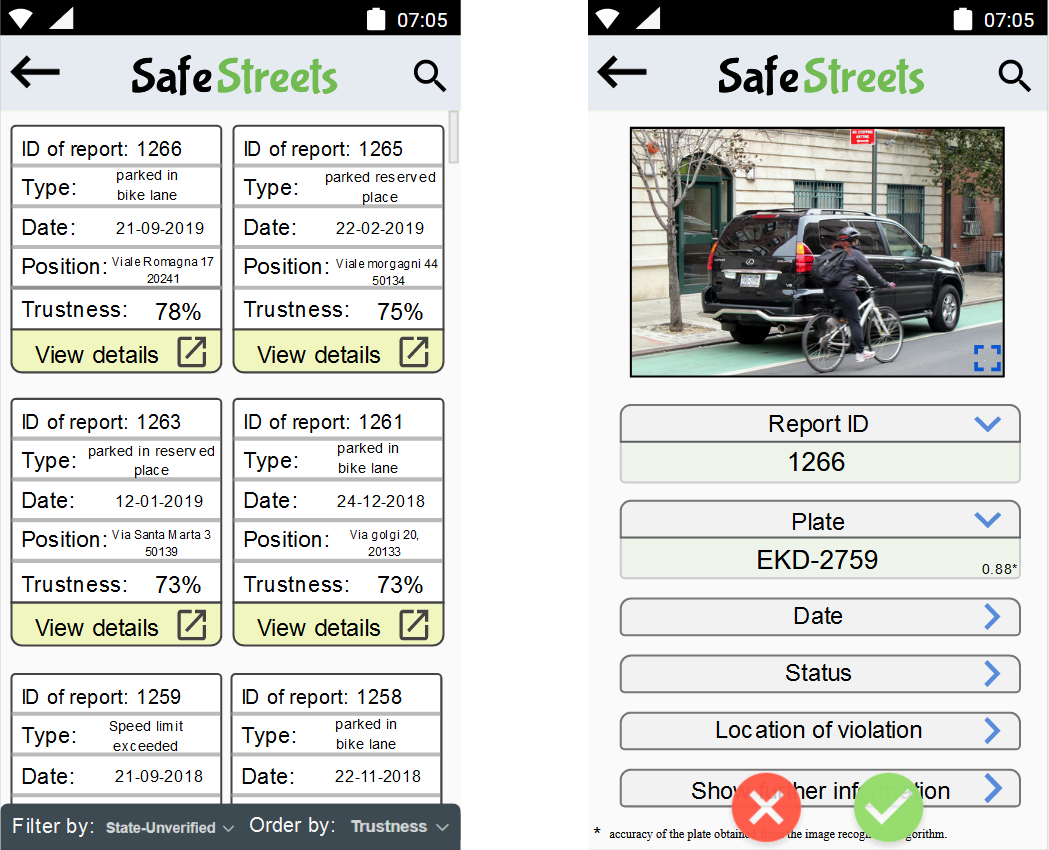
\includegraphics[scale=0.58]{Images/violations_and_details.png}
        \caption{Violations list interface}
    \end{figure}
    \newline\\
    \textbf{Details about a notification}\newline
    After an Authority clicks on \textit{View details} from the Violations list, he can access to details like license plate, model of the car, position where the violation occurred, the picture sent by the user, etc. The license plate of being shown is the output obtained from a image recognition algorithm, this output comes also with a number $\in [0,1]$ that represents the accuracy of the license plate obtained.
    \begin{figure}[h]
        \centering
        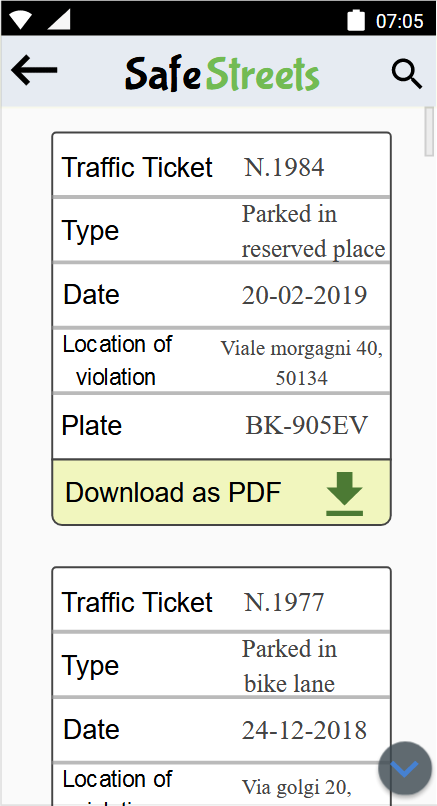
\includegraphics[scale=0.68]{Images/traffic_ticket.png}
        \caption{Traffic tickets interface}
    \end{figure}\newline\\
    \textbf{Traffic tickets generated}\newline
    In the previous activity it was possible to see that an Authority can press on $X$ button to reject a report from a user or to press on the check button to accept and  generate a traffic ticket related to it. In \textit{Figure 12} all the traffic tickets generated by the Authority logged in are shown, It is possible to download the traffic ticket as a PDF file.
    \newpage\vspace{3mm}
    \noindent\textbf{Get Suggestions}\newline
    \textit{Figure 10} shows the list of possible suggestions that authorities can see, each Authority see only the possible suggestions related to the own city, so this list can be shared between different districts but in the same city. An authority can print the suggestion by downloading as a PDF file or he/she can share it to the department in charge of receiving suggestions by citizens. The suggestions are taken from an AI algorithm  that is continuously updating its own dataset by modifying the effectiveness of each possible solution to each problem.  
    
       \begin{figure}[h]
        \centering
        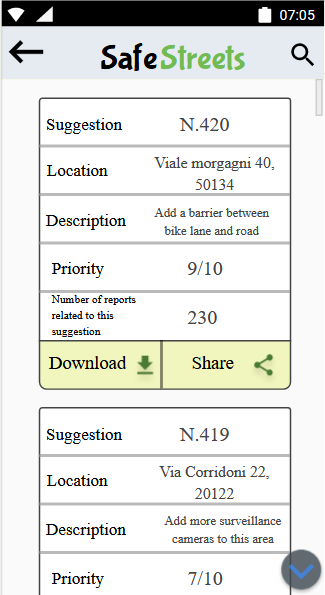
\includegraphics[scale=0.9]{Images/suggestions.png}
        \caption{Get suggestions interface}
    \end{figure}\vspace{5mm}
    \noindent\textbf{Statistics}\newline
    Users and Authorities can also see statistics about traffic violations and how SafeStreets impacts in streets safeness. An example is the graph \textit{Effectiveness of SafeStreets}, in this graph it is possible to see how the rate between traffic tickets generated and notifications sent has been increasing since the last years.  
       \begin{figure}[h]
        \centering
        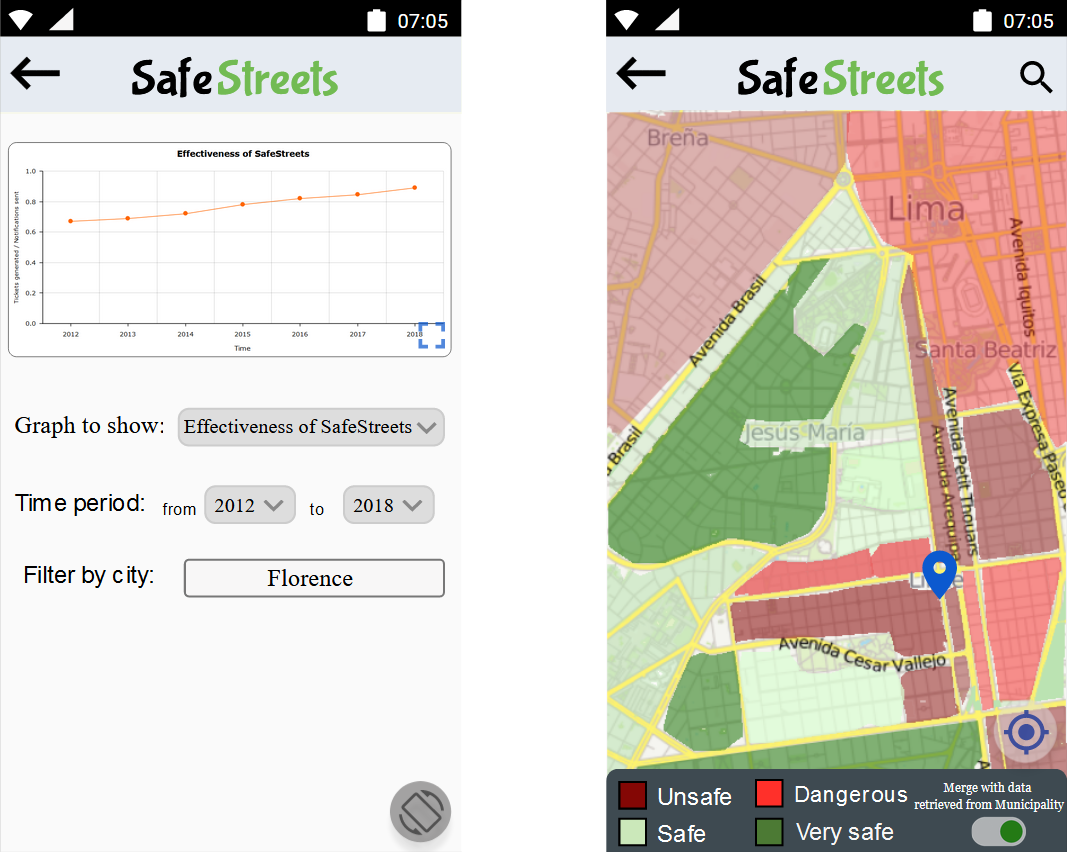
\includegraphics[scale=0.56]{Images/statistics_safe_unsafe2.png}
        \caption{Statistics and Safe/Unsafe Areas interface}
    \end{figure}\vspace{10mm}
    \newline\textbf{Areas with highest traffic violations}\newline
    This activity gives the possibility to see the tag assigned to each area in which SafeStreets has been used (or areas that are present in a service offered by the municipality). There are 4 possible labels: Safe, Unsafe, Very Safe and Dangerous. The tags inferred can be produced by merging the own data of SafeStreets with the data retreived from a service provided by the Municipality, if the option is enabled.
\subsubsection{Hardware Interfaces}
SafeStreets is available for smartphones that guarantee location data acquisition, access to the camera and internet access.
    \newpage
\subsubsection{Software Interfaces}
\begin{itemize}
    \item \textbf{Maps Service:} the system to be access to a map service that allows to show safe and unsafe areas.
    \item \textbf{Municipality Accidents History Service:} SafeStreets can cross its own data with the information provided by the Municipality Accidents History API to suggest possible interventions.
    \item \textbf{Municipality Traffic Tickets Service:} Municipality offers a service that allows to generate traffic tickets from the violations coming from SafeStreets. Safestreets sends information (confirmed as traffic violations) to the department in charge of generating traffic tickets in the municipality.
\end{itemize}

\subsubsection{Communication Interfaces}
The system uses HTTPS protocol to transmit data over the internet and to the DBMS.
\subsection{Functional Requirements}


\subsubsection{Use Cases}

% Use Case Diagrams

 \begin{figure}[H]
 \centering
        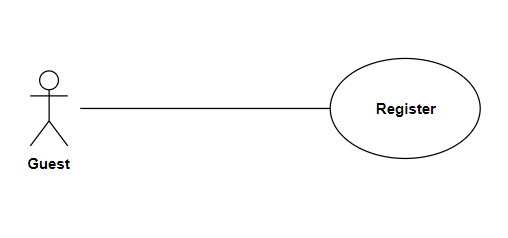
\includegraphics[width=0.7\textwidth]{Images/UCD_guest.PNG}
        \caption{Use Case Diagram: User}
    \end{figure}


 \begin{figure}[H]
        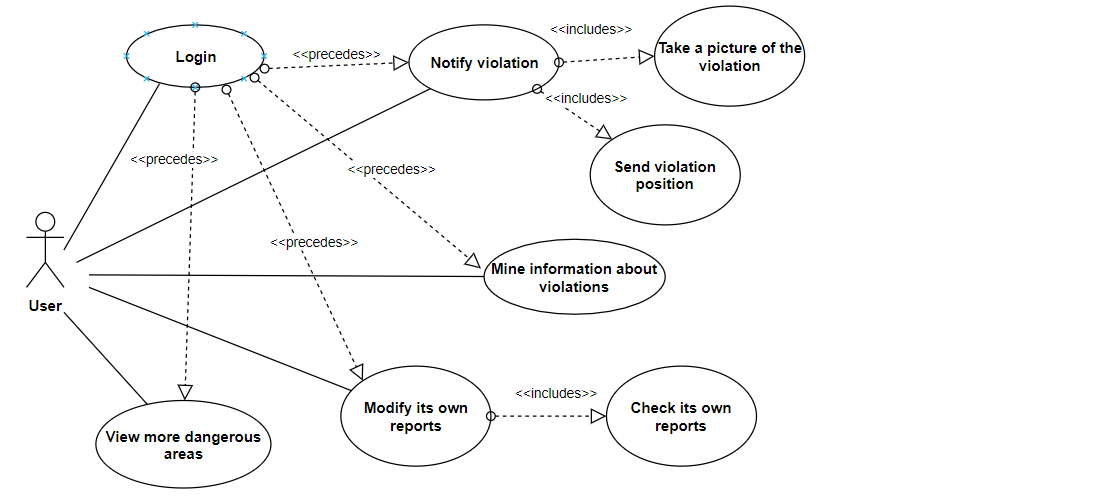
\includegraphics[width=1.5\textwidth,left]{Images/UCD_user_bis.PNG}
        \caption{Use Case Diagram: User}
    \end{figure}
    
    
    
    
     \begin{figure}[H]
          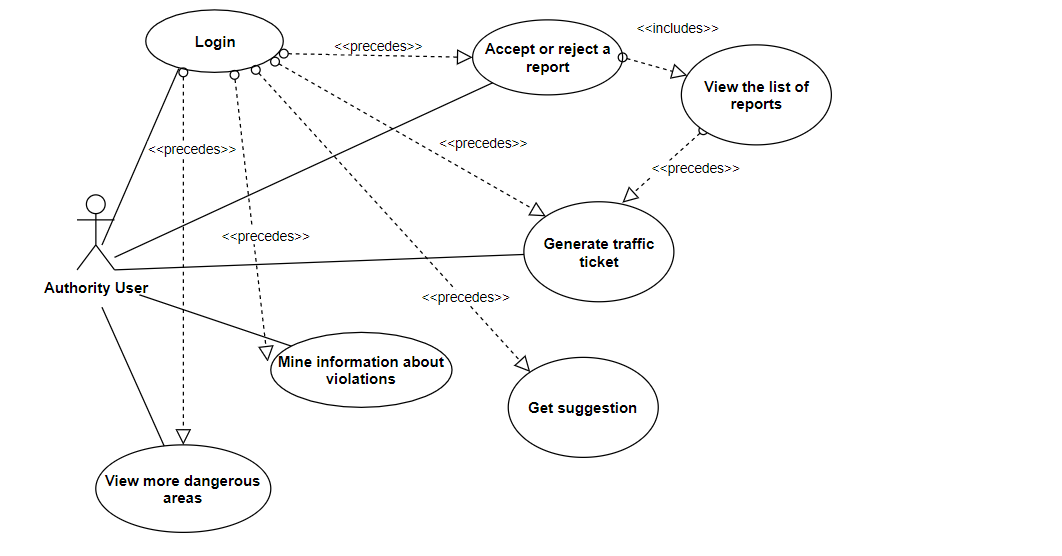
\includegraphics[width=1.5\textwidth,left]{Images/UCD_aut_bis.PNG}
        \caption{Use Case Diagram: Authority}
    \end{figure}


%Scenarios
\vspace{18mm}
\textbf{Scenarios:}\\\\
\textbf{Scenario 1}\\
Steven just decided he wants to stop using public services, and start going to the university by bike every morning, to save some money, and to boost his health conditions. But Milan is a tricky place where to hang around by bike, and Steven knows that he has to pay attention to the traffic, and to the large amount of cars that usually cross the bike lane, or park on it, forcing him to pass through the car road and putting him in danger. \\
In order to avoid those risky paths, Steven downloads \textit{SafeStreets}, creates an account, logs in, and accesses the information about violations stored by the application, to locate the most dangerous zones with relation to his problem. This allows him to choose the safest way (even if a little bit longer maybe) to get to the university from his place.\\\\

\noindent\textbf{Scenario 2}\\
As a consequence of popular protests due to bad urban conditions, the municipality of Firenze is in a situation in which, to accomplish the citizens and to raise the city liveability, must to bring some improvement to the urban infrastructure, but they don't know where to start because of a limited budget.\\
By using the \textit{SafeStreets} suggestion function, they can exploit the melting of their own information, crossed with the information that \textit{SafeStreets} stored in its lifetime about the violations. From all these information, \textit{SafeStreets} can suggest the municipality the best measures to implement to get the maximum urban situation improvement possibile.  \\

\noindent\textbf{Scenario 3}\\
Diane has a website in which she writes about social problems in her country, Peru. Her next article is about safeness, the solutions that each city has implemented problem and their effectiveness. She finds out that some municipalities decided to collaborate with a mobile application that involves citizens by allowing them to report traffic violations. During the investigation in which Diane was working on, she realizes that the cities that implemented it became safer and so she decides to use the statistics in \textit{SafeStreets} to show how many violations are being committed in each city that collaborated with the application and how effective is \textit{SafeStreets}.

%%%%%%%%  use casessssss %%%%%%%%%%%%%%%%%%%%%%%

\begin{table}[H]
\begin{tabular}{|l|p{0.9\textwidth}|}
\hline
\textbf{ID}             & UC1                                                                             \\ \hline
\textbf{Description}    & A \textit{Guest} creates a normal \textit{User} account to use the application \\ \hline
\textbf{Actors}         &   \textit{Guest}                                                                            \\ \hline

\textbf{Preconditions}  &   \begin{itemize}

 \item \textit{Guest} has downloaded the app onto his device
   \item      \textit{Guest} has a working internet connectivity
     \item       \textit{Guest} hasn't an account still.
                 \end{itemize}     
                    \\ \hline
                    
\textbf{Flow of Events} &   \begin{enumerate}
    \item The \textit{System} ask the \textit{Guest} to Log in or to Register
    \item The \textit{Guest} choose the Register option
    \item The \textit{System} return the registration form
    \item The \textit{Guest} fill in the form with its personal information and click confirm button
    \item The \textit{System} checks the validity of the input
    \item The \textit{System} generates a new account with a new identifier
    \item The \textit{System} sends a confirmation e-mail to the \textit{Guest}
\end{enumerate}                                                                             \\ \hline
\textbf{Postconditions} &  The \textit{Guest} becomes a \textit{User}, and is now able to log in and use the application services                                                                     \\ \hline

\textbf{Exceptions} &    \begin{itemize}
    \item The \textit{Guest} inputs a non-valid e-mail address
    \item The \textit{Guest} inputs a password that not matches with security standards. 
    \end{itemize} 
  In both cases, the \textit{System} will not let the confirm button to be pressed until all fields are correctly filled in.
                                                                            \\ \hline
\end{tabular}
\end{table}



%UC2




\begin{table}[H]
\begin{tabular}{|l|p{0.9\textwidth}|}
\hline
\textbf{ID}             & UC2                                                                             \\ \hline
\textbf{Description}    & A normal \textit{User} logs in \\ \hline
\textbf{Actors}         &   \textit{User}                                                                            \\ \hline

\textbf{Preconditions}  &   \begin{itemize}

 \item \textit{User} has downloaded the app onto his device
   \item      \textit{User} has a working internet connectivity
     \item       \textit{User} has an account
                 \end{itemize}     
                    \\ \hline
                    
\textbf{Flow of Events} &   \begin{enumerate}
    \item The \textit{System} ask the \textit{User} to Log in or to Register
    \item The \textit{User} choose the log in option
    \item The \textit{System} return the log in form
    \item The \textit{User} fill in the form with its log in data, and press the log in button
    \item The \textit{System} checks the validity and the matching of the inputs
    \item The \textit{User} accesses the interface with the various \textit{User} functions

\end{enumerate}                                                                             \\ \hline
\textbf{Postconditions} &  The \textit{User} is now able  to browse in the application and to use the application services                                                                     \\ \hline

\textbf{Exceptions} &    \begin{itemize}
    \item The \textit{User} inputs a non-existing username
    \item The \textit{User} inputs a wrong password for that username. 

\end{itemize}                                             The flow of the events restarts at point 4, showing an error message.                                \\ \hline

\end{tabular}
\end{table}


%UC3




\begin{table}[H]
\begin{tabular}{|l|p{0.9\textwidth}|}
\hline
\textbf{ID}             & UC3                                                                             \\ \hline
\textbf{Description}    & A normal \textit{User} notifies a violation \\ \hline
\textbf{Actors}         &  \textit{User, System}                                                                       \\ \hline

\textbf{Preconditions}  &   \begin{itemize}

 \item \textit{User} is logged in the application
                 \end{itemize}     
                    \\ \hline
                    
\textbf{Flow of Events} &   \begin{enumerate}
    \item The \textit{User} browses to the report violation section
    \item The \textit{System} return the form for reporting a violation
    \item The \textit{User} fill in the form with the mandatory data
    \item The \textit{User} press the button to take a picture of the violation
    \item The \textit{User} press the send button, and send the notification.
    \item The \textit{System} runs an algorithm to extract metadata about the notification, and to check the validity of the information. Then submits the report to the \textit{Authorities}.
    \item The \textit{System} add the report to the \textit{User} reports section. 

\end{enumerate}                                                                             \\ \hline
\textbf{Postconditions} & \begin{itemize}
     
 \item The \textit{User} can see the his/her new report and its status in the \textit{My Report} section. 
 
 \item The Authorities can see the notification in their report list
 \end{itemize}\\ \hline

\textbf{Exceptions} &    \begin{itemize}
    \item The \textit{User} inputs non valid data
    \item The \textit{User} doesn't input some mandatory data.

\end{itemize}
The send button will not be available until fields are correctly filled in.

\begin{itemize}
    \item The \textit{System} will find irregularities by running its algorithms.
\end{itemize}
In this case, the notification will be rejected.     
                           \\ \hline

\end{tabular}
\end{table}







%UC4





\begin{table}[H]
\begin{tabular}{|l|p{0.9\textwidth}|}
\hline
\textbf{ID}             & UC4                                                                             \\ \hline
\textbf{Description}    & A \textit{User} mines information about urban violations \\ \hline
\textbf{Actors}         & Normal  \textit{User}, Authority \textit{User}                                                                       \\ \hline

\textbf{Preconditions}  &   \begin{itemize}

 \item \textit{User} is logged in the application
                 \end{itemize}     
                    \\ \hline
                    
\textbf{Flow of Events} &   \begin{enumerate}
    \item The \textit{User} browses to the statistic section
    \item The \textit{System} return the form for searching for statistics
    \item The \textit{User} selects the information which he/she wants information about
    \item The \textit{User} press the search button 
    \item The \textit{System} shows the results of the search

\end{enumerate}                                                                             \\ \hline
\textbf{Postconditions} & \begin{itemize}
     
 \item The search parameters are cached in a preference list
 \end{itemize}\\ \hline

\textbf{Exceptions} &    \begin{itemize}
    \item No results exist for the search performed by the \textit{User}. So an advice is showed up.
   

\end{itemize}
  
                           \\ \hline

\end{tabular}
\end{table}







%UC5






\begin{table}[H]
\begin{tabular}{|l|p{0.9\textwidth}|}
\hline
\textbf{ID}             & UC5                                                                             \\ \hline
\textbf{Description}    & A \textit{User} checks and modify its own reports \\ \hline
\textbf{Actors}         & Normal  \textit{User}                                                                     \\ \hline

\textbf{Preconditions}  &   \begin{itemize}

 \item \textit{User} is logged in the application
                 \end{itemize}     
                    \\ \hline
                    
\textbf{Flow of Events} &   \begin{enumerate}
    \item The \textit{User} browses to the report list section
    \item The \textit{System} return the form with the list of the reports made by the \textit{User}
    \item The \textit{User} order the reports by some criteria, or search for some precise reports by the filter option. 
     \item The \textit{System} shows the results of the search
    \item The \textit{User} taps on the reports he/she wants to check
    \item The \textit{System} shows the report details.
    \item  The \textit{User} tap on modify button, and change the parameters of the report, or mark it as "canceled".
    \item The \textit{User} tap save button
   
\end{enumerate}                                                                             \\ \hline
\textbf{Postconditions} & \begin{itemize}
     
 \item The report is now changed.
 \item Authorities \textit{Users} can see which modifications has been made to the report.
 \item Authorities \textit{Users} can still see the reports marked as  "cancelled", and decide about them.
 \end{itemize}\\ \hline

\textbf{Exceptions} &    \begin{itemize}
    \item The \textit{User} didn't send any report still. So an empty list is showed up.
    \item The \textit{User} tries to modify a report that has been already accepted. The modification is not allowed, and the flow of events restart from event 6.
   

\end{itemize}
  
                           \\ \hline

\end{tabular}
\end{table}





%UC6




\begin{table}[H]
\begin{tabular}{|l|p{0.9\textwidth}|}
\hline
\textbf{ID}             & UC6                                                                             \\ \hline
\textbf{Description}    & An Authority \textit{User} validates a report \\ \hline
\textbf{Actors}         &  Authority \textit{User}                                                                       \\ \hline

\textbf{Preconditions}  &   \begin{itemize}

 \item Authority \textit{User} is logged in the application
                 \end{itemize}     
                    \\ \hline
                    
\textbf{Flow of Events} &   \begin{enumerate}
    \item The authority \textit{User} browses to the reports list section
    \item The \textit{System} return the list of reports from normal \textit{Users}
    \item The authority \textit{User} filters and orders the reports according to his/her needs
    \item The authority \textit{User} taps on the chosen report
    \item The authority \textit{User} taps the validate green button.

\end{enumerate}                                                                             \\ \hline
\textbf{Postconditions} & \begin{itemize}
     
 \item The report is now marked as "validated", and it is officially a violation
 \item The \textit{User} who sent the report can no longer modify it 
 \end{itemize}\\ \hline

\textbf{Exceptions} &    \begin{itemize}
    \item There are no reports in a "to be seen" status
   

\end{itemize}
  
                           \\ \hline

\end{tabular}
\end{table}




%UC7





\begin{table}[H]
\begin{tabular}{|l|p{0.9\textwidth}|}
\hline
\textbf{ID}             & UC7                                                                             \\ \hline
\textbf{Description}    & An Authority \textit{User} rejects a report \\ \hline
\textbf{Actors}         &  Authority \textit{User}                                                                       \\ \hline

\textbf{Preconditions}  &   \begin{itemize}

 \item Authority \textit{User} is logged in the application
                 \end{itemize}     
                    \\ \hline
                    
\textbf{Flow of Events} &   \begin{enumerate}
    \item The authority \textit{User} browses to the reports list section
    \item The \textit{System} return the list of reports from normal \textit{Users}
    \item The authority \textit{User} filters and orders the reports according to his/her needs
    \item The authority \textit{User} taps on the chosen report
    \item The authority \textit{User} taps the reject red button.

\end{enumerate}                                                                             \\ \hline
\textbf{Postconditions} & \begin{itemize}
     
 \item The report is now marked as "rejected", and so it is not a violation
 \item The \textit{User} who sent the report can no longer modify it 
 \end{itemize}\\ \hline

\textbf{Exceptions} &    \begin{itemize}
    \item There are no reports in a "to be seen" status
   

\end{itemize}
  
                           \\ \hline

\end{tabular}
\end{table}





%UC8






\begin{table}[H]
\begin{tabular}{|l|p{0.9\textwidth}|}
\hline
\textbf{ID}             & UC8                                                                           \\ \hline
\textbf{Description}    & An Authority \textit{User} generates a traffic ticket \\ \hline
\textbf{Actors}         &  Authority \textit{User}                                                                       \\ \hline

\textbf{Preconditions}  &   \begin{itemize}

 \item Authority \textit{User} is logged in the application
                 \end{itemize}     
                    \\ \hline
                    
\textbf{Flow of Events} &   \begin{enumerate}
    \item The authority \textit{User} browses to section for generating tickets
    \item The \textit{System} return the form the fill in for generating a ticket
    \item The authority \textit{User} fills in the form, with all data and link the ticket to the relative reports (o comunque una roba del genere)
    \item The authority \textit{User} clicks the generate button

\end{enumerate}                                                                             \\ \hline
\textbf{Postconditions} & \begin{itemize}
     
 \item A new ticket now exists in the authorities database, and it will be sent to the right recipient.
 \item The status of the report in relation with this ticket will change in "processed". (o qualcosa che indica che per quel report è già stata fatta una multa)
 \end{itemize}\\ \hline

\textbf{Exceptions} &    \begin{itemize}
    \item The authority \textit{User} doesn't fill in some field, or fill it in a wrong way.
\end{itemize}

When "generate" button is pressed, the \textit{System} will shows up an alert message, and the flow of the events will restart from event 3

\begin{itemize}
    \item The authority \textit{User} links the ticket with a violation whose involved license plates or vehicles are not the same included in the generated ticket.
\end{itemize}
   The \textit{System} will shows up an alert message, and the flow of the events will restart from event 3
  
\begin{itemize}
    \item The authority \textit{User} links the ticket with a report which is not in a "validated" state.
\end{itemize}
   The \textit{System} will shows up an alert message, and the flow of the events will restart from event 3
                           \\ \hline

\end{tabular}
\end{table}






%UC9




\begin{table}[H]
\begin{tabular}{|l|p{0.9\textwidth}|}
\hline
\textbf{ID}             & UC9                                                                           \\ \hline
\textbf{Description}    & An Authority \textit{User} searches for a suggestion \\ \hline
\textbf{Actors}         &  Authority \textit{User}                                                                       \\ \hline

\textbf{Preconditions}  &   \begin{itemize}

 \item Authority \textit{User} is logged in the application
 \item Involved municipality must provide an interface to share its data stored with \textit{SafeStreets System}
                 \end{itemize}     
                    \\ \hline
                    
\textbf{Flow of Events} &   \begin{enumerate}
    \item The authority \textit{User} browses to the suggestions section
   
   \item The \textit{system} retrieves the list of suggestions
   \item The authority \textit{User} clicks on search button
   \item The authority \textit{User} inserts the keywords he/she wants to look for
   \item The \textit{System} retrieves che list of filtered suggestions
    \item The authority \textit{User} clicks on the suggestion he wants to look at and share
    \item The \textit{System} shows all the detail of the suggestion
    \item The authority \textit{User} clicks on the share option
    \item The \textit{System} pops up a window from which to chose where to share the suggestion

\end{enumerate}                                                                             \\ \hline
\textbf{Postconditions} & \begin{itemize}
     
 \item None
 \end{itemize}\\ 
 \hline

\textbf{Exceptions} &    \begin{itemize}
   
   \item No suggestions match the keywords specified. In this case, no results are showed, and a alert message show up

\end{itemize}
  
                           \\ \hline

\end{tabular}
\end{table}

%%%%%%%%%%%%%% fine use casesss %%%%%%%%%%%%%
\newpage
\subsubsection{Sequence Diagrams}
    \begin{figure}[H]
        \centering
        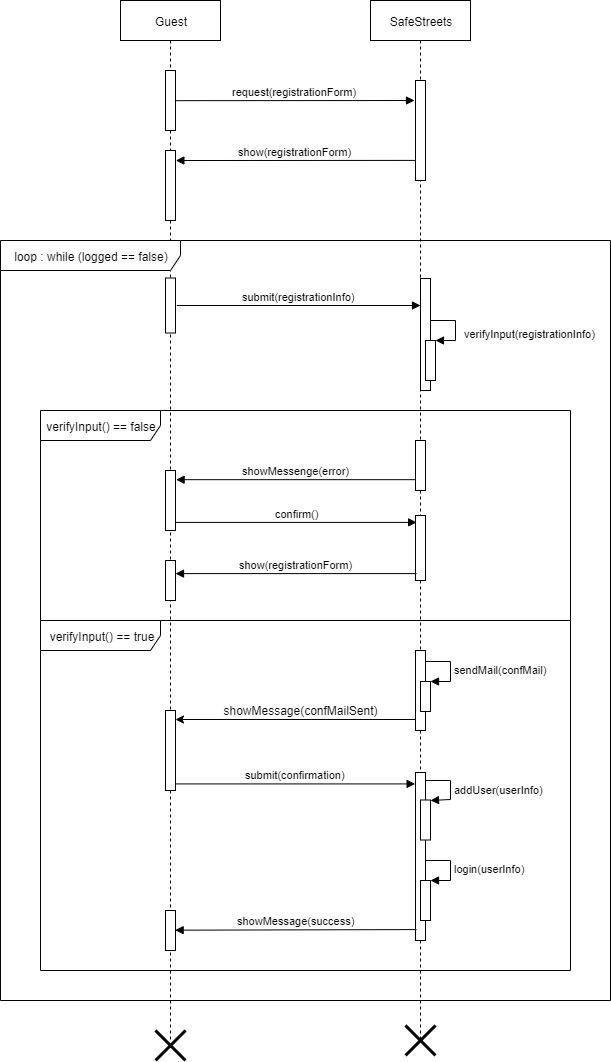
\includegraphics[scale=0.5]{Images/SeqDiag_registration.png}
        \caption{Sequence Diagram of the registration of a User}
    \end{figure}
    
    \begin{figure}[H]
        \centering
        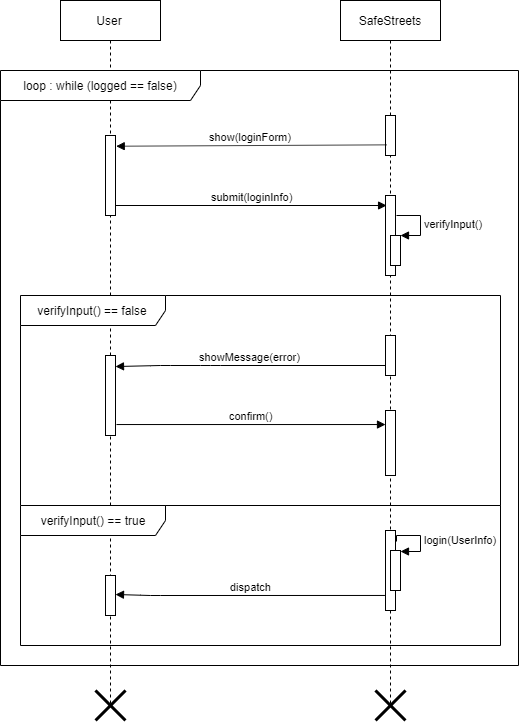
\includegraphics[scale=0.5]{Images/SeqDiag_login.png}
        \caption{Sequence Diagram of the login of a User or of an Authority}
    \end{figure}
    
    \begin{figure}[H]
        \centering
        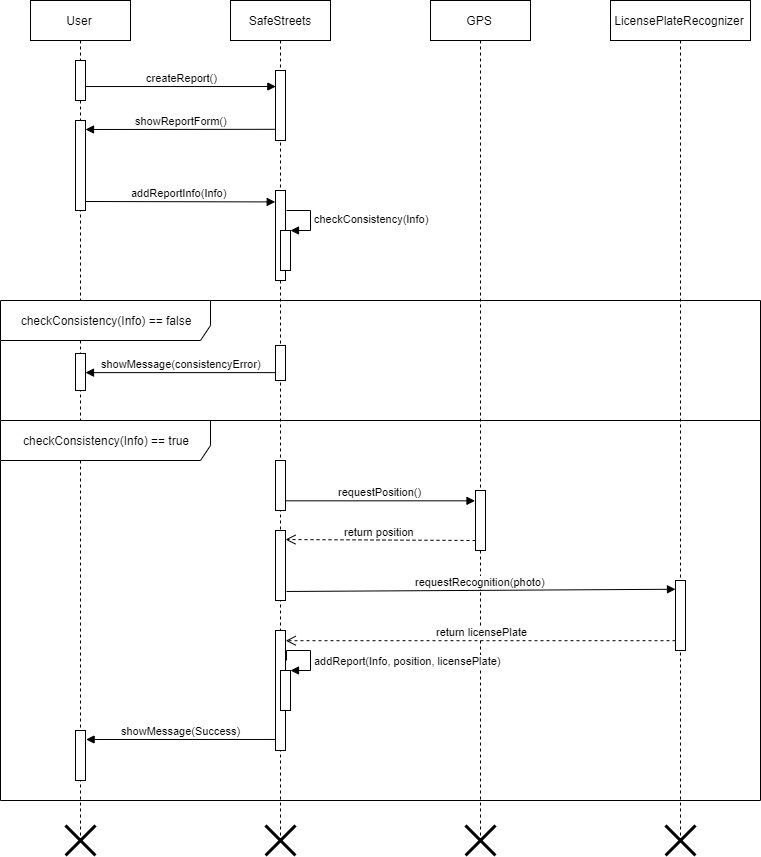
\includegraphics[scale=0.5]{Images/SeqDiag_addReport.png}
        \caption{Sequence Diagram of the insertion of a Report by a User}
    \end{figure}
    
    \begin{figure}[H]
        \centering
        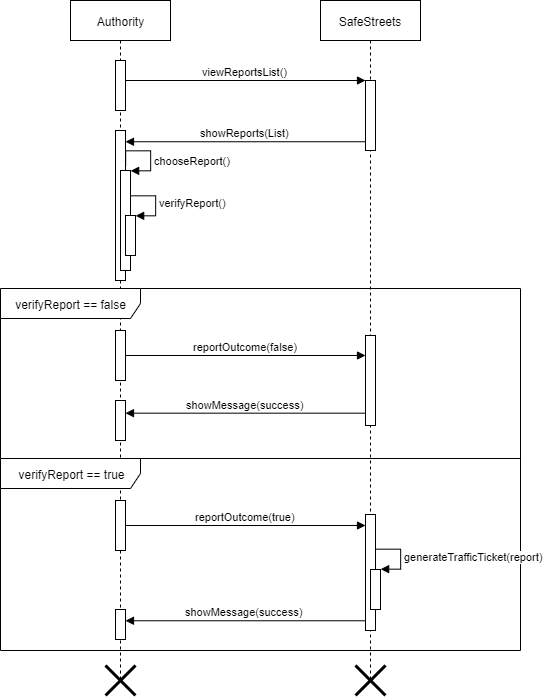
\includegraphics[scale=0.5]{Images/SeqDiag_generateTrafficTicket.png}
        \caption{Sequence Diagram of the checking of a Report and, eventually, the generation of the corresponding Traffic Ticket}
    \end{figure}
    
    \begin{figure}[H]
        \centering
        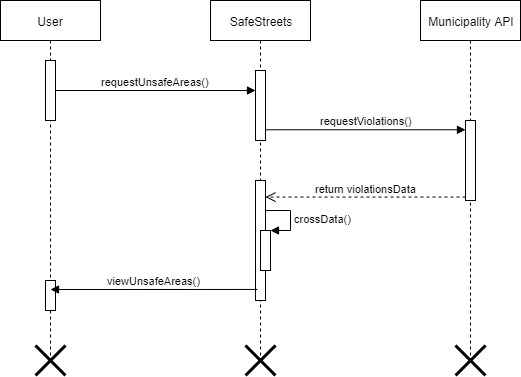
\includegraphics[scale=0.5]{Images/SeqDiag_unsafeAreas.png}
        \caption{Sequence Diagram of the request to know which are the unsafe areas}
   \end{figure}
\subsubsection{Goal mapping on requirements}






In this section, it will be showed the functional requirements and the domain assumption related to each goal.
\begin{itemize}


\item \textbf{{[G.1]} Allows the User to access the functionalities of the application from different locations and devices.}
\begin{itemize}
    \item \textbf{[R.1]}A \textit{guest} must be able to register and become a \textit{User}.
    
     \item \textbf{[R.2]} The S2B must provide an already created account to the \textit{Authorities}.
    
    \item \textbf{[R.3]} The S2B must check that credentials are correct, then send a confirmation e-mail.
    
     \item \textbf{[R.4]}The S2B must check the validity of the document sent by a \textit{User} to give his/her the access to all the functionalities.
     
      \item \textbf{[R.5]}The S2B must allow \textit{User} to log in with his/her registration credentials.
      
       \item \textbf{[D.1]}Personal data given by Users during the registration process are assumed to be correct.
\end{itemize}

\item \textbf{{[G.2]} Allows the \textit{User} to notify about traffic violations.}
\begin{itemize}
        \item \textbf{[R.5]}The S2B must allow \textit{User} to log in with his/her registration credentials.
        
        \item \textbf{[R.6]}The S2B must provide an algorithm for compute the trustness of reports.
        
        \item \textbf{[R.7]}\textit{User} must be allowed to see the list of his/her reports.
        
        \item \textbf{[R.8]}\textit{User} must be allowed to edit or cancel his/her reports. 
        
        \item \textbf{[R.9]}The S2B must allow the \textit{User} to send the report only within 5 minutes from when he/she starts to fill it in. 
        
        \item \textbf{[R.10]}The S2B must submit the received reports to an \textit{Authority} for checking its validity.
        
        \item \textbf{[R.11]}The S2B must recognize if a notification that is about to be made, may involve a violations already notified, and alert the \textit{User}
        
        \item \textbf{[R.12]}The S2B must recognize if more done reports refer to the same violation.
        
        \item \textbf{[D.3]} Pictures sent by Users are assumed to be in some precise file format.
        
        \item \textbf{[D.4]} The GPS is assumed to be subject to some precision error.
\end{itemize}

\item \textbf{{[G.3]} Allows the User to send pictures, type of the violation, license plate and time.}

\begin{itemize}
        \item \textbf{[R.13]} The S2B must allow the \textit{User} to only send pictures taken while filling in the notify form, accessing the camera by the \textit{SafeStreets} application, and not to upload some by the gallery.
        
        \item \textbf{[R.14]} The S2B must allows the \textit{User} to chose from a predefined list of "type of violation". 
        
        \item \textbf{[R.15]}The S2B must allow the \textit{User} to only send time automatically taken from the operative system timer.
        
        \item \textbf{[D.3]} Pictures sent by Users are assumed to be in some precise file format.
\end{itemize}


\item \textbf{{[G.4]} Must compute license plate, position and address from the received data.}

    \begin{itemize}
        
         \item \textbf{[R.9]}The S2B must allow the \textit{User} to send the report only within 5 minutes from when he/she starts to fill it in. 
         
        \item \textbf{[R.16]}The S2B must use some out coming map service.
        
         \item \textbf{[D.3]} Pictures sent by Users are assumed to be in some precise file format.
         
        \item \textbf{[D.4]} The GPS is assumed to be subject to some precision error.
    \end{itemize}
    
    
    
\item \textbf{{[G.5]} Allows Authority to check the correctness of a report.}

    \begin{itemize}
         \item \textbf{[R.2]} The S2B must provide an already created account to the \textit{Authorities}.
        
        \item \textbf{[R.5]}The S2B must allow \textit{User} to log in with his/her registration credentials.
        
        \item \textbf{[R.17]}The S2B must allow only 1 \textit{Authority} per time to change the status of a report.
        
        \item \textbf{[R.18]}The S2B must submit to the \textit{Authority} only the reports with a computed trust value higher than 60%.
        
    \end{itemize}
    
    
\item \textbf{{[G.6]} Allows Authority to generate traffic tickets from verified reports.}

    \begin{itemize}
    
        \item \textbf{[R.2]} The S2B must provide an already created account to the \textit{Authorities}.
        
         \item \textbf{[R.19]}The S2B must not allow \textit{Authority} to generate more tickets for the same violation
         
         \item \textbf{[R.20]}The S2B must allow generated tickets information to be moved into the \textit{Authorities} data store.
        
        \item \textbf{[D.5]} Violations for which a ticket is generated are supposed to be validated by authorities first.
        
    \end{itemize}


\item \textbf{{[G.7]} Allows both User and Authority to access information about unsafe areas.}
    \begin{itemize}
         \item \textbf{[R.2]} The S2B must provide an already created account to the \textit{Authorities}.

        \item \textbf{[R.5]}The S2B must allow \textit{User} to log in with his/her registration credentials.
        
        \item \textbf{[R.21]}The S2B must update the information about statistics and safe areas with the new validate reports within 10 seconds from the new information delivery.
    \end{itemize}
    
\item \textbf{{[G.8]} Allows both User and Authority to access statistics about effectiveness of SafeStreets.}

    \begin{itemize}
         \item \textbf{[R.2]} The S2B must provide an already created account to the \textit{Authorities}.

        \item \textbf{[R.5]}The S2B must allow \textit{User} to log in with his/her registration credentials.
        
        \item \textbf{[R.21]}The S2B must update the information about statistics and safe areas with the new validate reports within 10 seconds from the new information delivery.
        
    \end{itemize}
    
\item \textbf{{[G.9]} Allows both User and Authority to access statistics about violations.}
     \begin{itemize}
         \item \textbf{[R.2]} The S2B must provide an already created account to the \textit{Authorities}.

        \item \textbf{[R.5]}The S2B must allow \textit{User} to log in with his/her registration credentials.
        
        \item \textbf{[R.21]}The S2B must update the information about statistics and safe areas with the new validate reports within 10 seconds from the new information delivery.
        
    \end{itemize}
    
    
\item \textbf{{[G.10]} Must cross its data with the municipality ones in order to provide suggestions to improve urban mobility.}
    \begin{itemize}
        
         \item \textbf{[R.22]}SB2 must have been provided with the access authorization to the municipality data.
         
         \item \textbf{[R.23]}The S2B must check the physical feasibility of the suggestions provided, with relation to the map.
         
         \item \textbf{[R.24]}The S2B must generate suggestions based on the actual information and the actual urban situation.
       
         \item \textbf{[D.6]} Information obtained by authorities are    supposed to be correct.
         
         \item \textbf{[D.7]} Is assumed that there's no bounds which suggestions provided by the S2B have to respect.
          
    \end{itemize}
    
\item \textbf{{[G.11]} Must ensure that corrupted information are discarded.}
    \begin{itemize}
        \item \textbf{[R.25]}The S2B must use an algorithm to recognize picture that have been physically or digitally modified.
        
        \item \textbf{[R.26]}The S2B must compare received data with the ones computed with algorithms in order to find discrepancies.
        
        \item \textbf{[R.27]}The S2B must not submit to \textit{Authorities} the reports that have been valuated with a low trust level.
    \end{itemize}
\end{itemize}


\subsection{Performance Requirements}
This section contains some numerical requirements of the system, relative to the interaction with \textit{Users} and to the performances.
When a \textit{User} send a report, this must be taken in account (accepted or rejected) within one month by the competent authorities, and than another month to eventually generate a ticket. Due to DBMS storage issues, it's not possible to permanently store all the reports that does not lead to a "conclusion".\\
When a report is accepted by authorities, its existence must be take into account by the statistics functionalities in less than 30 seconds, in order to offer information and statistics always up to the most recent date.\\
A suggestion must be provided by \textit{SafeStreets} within the time span in which this suggestion can be useful and significant. \\
A report by a \textit{User} must be sended to \textit{SafeStreets} within 5 minutes from when the report has been created and the \textit{User} started to fill it. This comes with the intention of not allow \textit{User} to send wrong position by moving away from the violation location while compiling the form, or to send wrong time information.
\subsection{Design
Constraints}

\subsubsection{Standards compliance}
The system doesnt need to be directly compliant to any particular standard, it only needs to consider the position acquired from the User as \textit{Latitude} and \textit{Longitude}. In the design analysis it will be decided if it is necessary to add any further compliance.
\subsubsection{Hardware limitations}
\textit{SafeStreets} is a software application, the device with \textit{SafeStreets} installed must guarantee access to internet, a camera with at least 8 Megapixel and flash in order to take photos during night. 
\subsubsection{Any other constraint}
Each User must upload a photo of his/her ID document in order to have their account verified.
\subsection{Software System Attributes}

\subsubsection{Reliability}
\textit{SafeStreets} should be available 24/7 in order to allow Users to report traffic violations at any given time. However it can be accepted to have periods of 2-4 hours in which the server is down because of maintenance, this doesn't represent a problem since the mobile application can use a local Database and store the reports being sent by the User when it is down.
\subsubsection{Availability}
Since \textit{SafeStreets} does not have a critical nature, 90\% of availability is sufficient.
\subsubsection{Security}
In order to guarantee a secure system, \textit{SafeStreets} uses HTTPS for a secure communication between Users and the Server, HTTPS allows to avoid possible Man in the Middle attacks. However any other protocol or encryption algorithm will be discussed in the Design Document.
\subsubsection{Maintainability}
The System will follow good software engineering practices to allow maintainability, for example it is possible to use a local Database in order to allow the maintenance of the global database server. However, this will be discussed in the Design Document.
\subsubsection{Portability}
\textit{SafeStreets} is developed as a Web Application, it is sufficient to have a mobile phone that allows the use of web browsers. Thus, \textit{SafeStreets} has a maximum grade of portability.
